\documentclass[12pt,a4paper,oneside,article]{memoir}

% LAYOUT
\setulmarginsandblock{0.7\uppermargin}{0.8\lowermargin}{*}
\usepackage{mylayout}


% LANGUAGE AND FONT
\setmainlanguage{english}
\setmainfont[Ligatures={TeX},Mapping={tex-text},Numbers={OldStyle}]{Linux Libertine O}
\setmonofont[Scale=0.8]{DejaVu Sans Mono}

% PDF SETUP
\usepackage[unicode,bookmarks, colorlinks, breaklinks,
pdftitle={S-114.4202: Exercise report},
pdfauthor={Ville Väänänen},
pdfproducer={xetex}
]{hyperref}
\hypersetup{linkcolor=black,citecolor=black,filecolor=black,urlcolor=MidnightBlue} 

\usepackage[shadow]{todonotes}

% MATH
\usepackage{mymath}
\everymath{\displaystyle}

\usepackage{listings}
\lstset{ %
	language=R,                % choose the language of the code
	basicstyle=\footnotesize\ttfamily,% the size of the fonts that are used for the code 
	numbers=none,                   % where to put the line-numbers
	numberstyle=\footnotesize\ttfamily,      % the size of the fonts that are usedfor the line-numbers 
	stepnumber=5,                   % the step between two line-numbers. If it's 1 each line 
	aboveskip=2\medskipamount,
	belowskip=2\medskipamount,                                % will be numbered
	numbersep=-5pt,                  % how far the line-numbers are from the code
	backgroundcolor=\color{white},  % choose the background color. You must add \usepackage{color}
	showspaces=false,               % show spaces adding particular underscores
	showstringspaces=false,         % underline spaces within strings
	showtabs=false,                 % show tabs within strings adding particular underscores
	frame=l,
	framesep=0pt,
	framexleftmargin=2mm,
	rulecolor=\color{light-gray},	                % adds a frame around the code
	tabsize=2,	                % sets default tabsize to 2 spaces
	caption=,
	captionpos=t,                   % sets the caption-position to bottom
	breaklines=true,                % sets automatic line breaking
	breakatwhitespace=false,        % sets if automatic breaks should only happen at whitespace
	emptylines=*1,
	keywordstyle=\color[rgb]{0,0,1},          % keywords in blue
    commentstyle=\color[gray]{.5}\itshape,               % comments
    stringstyle=\color[rgb]{.627,.126,.941},   % strings in purple
	%title=\lstname,                 % show the filename of files included with
	                                % also try caption instead of title
	escapeinside={\%*}{*)},         % if you want to add a comment within your code
            % if you want to add more keywords to the set
}

\newcommand{\Th}{\gv{\theta}}
\newcommand{\LH}{\Pdf{\v{Y}}{\Th}}
\newcommand{\LHf}[1]{\Pdf{\v{Y}}{#1}}
\newcommand{\LHh}{\Pdf{\v{Y}}{\hat{\Th}}}
\newcommand{\lLH}{L\!\left(\Th\right)}
\newcommand{\cLH}{\Pdf{\v{X},\v{Y}}{\Th}}
\newcommand{\lcLH}{\log\cLH}
\newcommand{\LB}{\mathcal{L}}
\newcommand{\Lb}{\mathfrak{L}}
\newcommand{\KL}[2]{\mathrm{KL}\left(#1\|#2\right)}


\newcommand{\course}{S-114.4202}
\newcommand{\coursename}{Special Course in Computational Engineering II}
\newcommand{\duedate}{\today}
\newcommand{\studentid}{63527M}
\renewcommand{\title}{Bear observations in Finland in 2010}
\author{Ville Väänänen}

% SECTION NUMBERING
%\setsecnumdepth{subsubsection}
\counterwithout{section}{chapter}
%\renewcommand{\thesubsubsection}{\thesubsection{\large\scshape\alph{subsubsection}}}
%\titleformat{\subsubsection}{\large\scshape}{\alph{subsubsection} )}{10pt}{}
%\titleformat{\section}{\Huge}{\thesection}{10pt}{}
%\titleformat{\subsection}{\Large}{\thesubsection}{10pt}{}


% BIBLIOGRAPHY
\usepackage[hyperref=true,  backend=biber]{biblatex} % TEXLIPSE BUG: backend cannot be first
\addbibresource{/Users/dennari/Documents/Bibtex/Bear_data.bib}

\checkandfixthelayout

\begin{document}



\mytitlepage

\section{Data description}

The bear observations in the year 2010 are plotted in figure~\ref{fig:bear}
and the population density of the municipalities (the number of people
in the municipality per its land area) is plotted in figure~\ref{fig:pdens}. 
As can be seen, there is some clustering which has to be associated with increased
probability of reporting due population density. Thus an interesting problem is,
how should we take into account the probability for an animal to get observed
in a given area? Is it directly proportional to population density? Is there some
other factors associated such as the amount of hunters in the area?

\begin{figure}[htbp]
  \begin{adjustwidth}{-2in}{-2in}
	  \centering
	  \subfloat[Bear observations in 2010]{\label{fig:bear}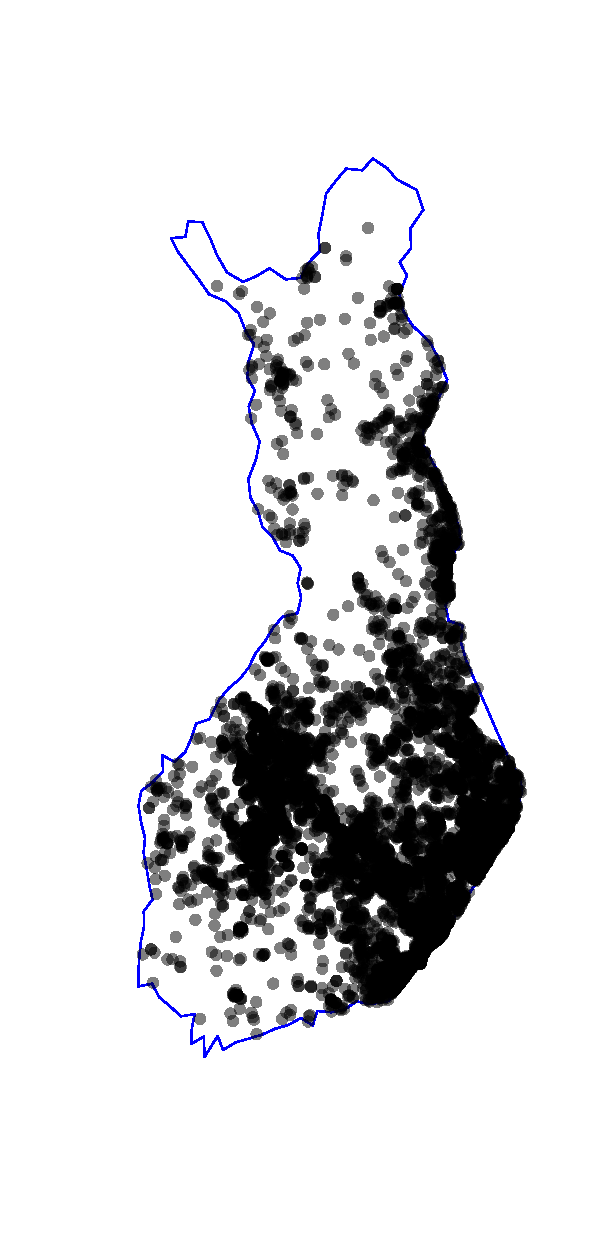
\includegraphics[width=0.6\textwidth]{b2010}}
	  \subfloat[Population density]{\label{fig:pdens}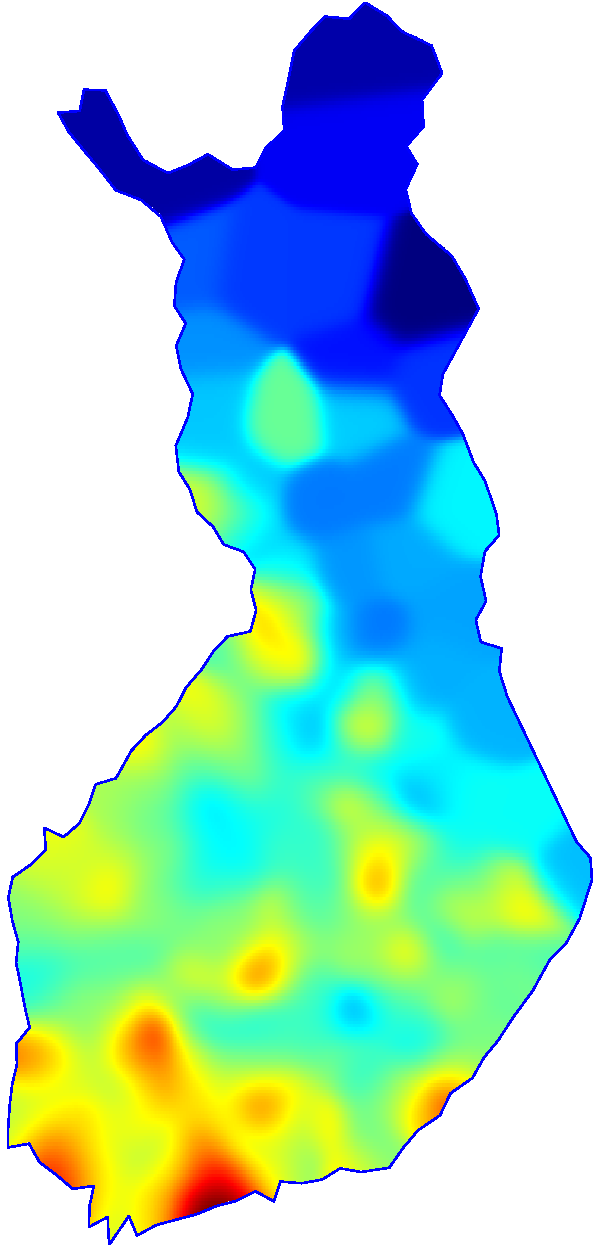
\includegraphics[width=0.6\textwidth]{pdens}}
  \end{adjustwidth}
  \caption{Bear observations in 2010 and the population density of Finland}
  \label{fig:bw2010}
\end{figure}


\section{Methods}

\subsection{Cox processes}

Cox processes
are a broad class of point processes that are nonhomogoneous Poisson processes given
a \emph{latent random intensity field} $\lambda(\v{s})$. Throughout the report, we will denote 
vectors and vector valued functions with bold lower-case symbols and matrices with bold
upper case symbols. We will denote a \emph{spatial point process} defined in some bounded region $\Omega\subset\R^2$, 
also called the \emph{observation window}, with $\mathcal{Y}(\v{s})$ where $\v{s}\in\Omega$.
A realisation of a point process is called a \emph{point pattern}
\begin{align}
	\v{y}=\left[\mathcal{Y}(\v{s}_1),\dots,\mathcal{Y}(\v{s}_n)\right]^T,
	\label{eq:point_pattern}
\end{align}
that can be thought of as an $n$ dimensional random vector governed by a well defined
multivariate distribution \cite{Gelfand2010}. It is important to realise that
the elements of $\v{y}$ belong to some abstract sample space, i.e. bears or wolves
in case of this report \cite{Gelfand2010}. Also, \eqref{eq:point_pattern}
implicitly defines a matrix $\v{S}=\left[\v{s}_1, \dots, \v{s}_n\right]$ of
point locations.

Going back to Cox processes, given the intensity field, the number of points $N(D)$ inside a region $D\subset\Omega$ 
is a Poisson distributed random variable with mean $\Lambda(D)=\defint{D}{}{\lambda(\v{s})}{\v{s}}$, i.e.
\begin{align}
	\Pdf{N(D)=k}{\Lambda(D)}=\frac{\Lambda(D)^k}{k!}e^{-\Lambda(D)^k}.
	\label{eq:poisson}
\end{align}
In a log-Gaussian Cox process, the latent intensity field has the form
\begin{align}
	\lambda(\v{s})&=\exp\left(Z(\v{s})\right)
	\label{eq:lambda_lgcp}
\end{align}
where $Z$ is a \emph{Gaussian random field} (also called a Gaussian process, GP) defined by a 
mean function $\mu(\v{s})$ and a covariance function $Q(\v{s},\v{s}')$ \cite{Moller2007}. 
In this report
a linear model will be used for the mean function, i.e
\begin{align}
	\E{\log\lambda(\v{s})}&=\gv{\beta}^T\v{z},
	\label{eq:lambda_mean}
\end{align}
where typically $z_1(\v{s})=1$, so that $\beta_1$ is the intercept. With this definition, possible
covariate data can be included directly in $\v{z}$. 

% The complete set of unknown parameters in our model
% is then
% \begin{align}
% 	\gv{\theta}&=\left[\gv{\theta}_Q^T,\;\gv{\beta}^T\right]^T
% 	\label{eq:parameters}
% \end{align}

\subsection{Latent Gaussian models}

Our aim is to be able to use a computationally efficient Bayesian procedure for inference
in latent Gaussian models called INLA (or integrated nested Laplace approximations) \cite{Rue2009}.
Latent Gaussian models are a large set of flexible models, where given a realisation $\v{x}$ 
of a latent (unobserved) Gaussian random field the observations $\v{y}$ are independent and identically
distributed. 
More precisely we have
\begin{align}
	Z(\v{s})|\gv{\theta}&\sim \mathcal{GP}(\mu(\v{s},\gv{\theta}),Q(\v{s},\v{s}',\gv{\theta})\\
	\v{y}|Z(\v{s}),\gv{\theta}&\sim \prod_{k=1}^n \Pdf{y_k}{Z(\v{s}),\gv{\theta}} \label{eq:latent_gaussian_clh}
\end{align} 
Here we have introduced the hyperparameter $\gv{\theta}$. It is worth noting that
in this vector notation $\v{x}$ has to be thought of as belonging to an infinite
dimensional Hilbert space. 

\subsection{Likelihood approximation}

LGCP's can be thought of as latent Gaussian models and in their case the logarithm of the 
conditional likelihood function
\eqref{eq:latent_gaussian_clh} can be written as \cite{Moller2007,Gelfand2010,Simpson2011} (going further, dependence on the hyperparameter
will be suppressed but is assumed)
\begin{align}
	\log\Pdf{\v{y}}{Z}&= \abs{\Omega}-\defint{\Omega}{}{e^{Z(\v{s})}}{\v{s}}+\sum_{k=1}^n Z(\v{s}_k)
	\label{eq:lgcp_clh}
\end{align} 
Unfortunately \eqref{eq:lgcp_clh} cannot be evaluated without first forming some kind of
approximation to the latent random field $Z(\v{s})=\log \lambda(\v{s})$. With the help of such an approximation, the last term requires
just the evaluation of the approximated field in the observed locations. Since the integral of the intensity
function over the observation window (i.e. the mean number of points in the pattern) will remain 
analytically intractable it will be computed numerically \cite{Simpson2011}.

A common approach for approximating the conditional likelihood is to partition the observation window
to a regular grid and assume the field constant inside a grid cell. The value chosen for a cell
can $c_{k}$ be for example the value of the field in the cell's center point $\v{c}_k$. Clearly in this case
the number of points in a grid cell is Poisson distributed with mean $\abs{c_{k}}e^{Z(\v{c}_k)}$.
As argued in \cite{Simpson2011} it is far from optimal to use the grid both for approximating
the intensity field \emph{and} the locations of the points $y_k$. A nicer alternative would be to 
form a finite dimensional \emph{continous} approximation to the field, so that it could be evaluated at 
the exact point locations.

This can be achieved by forming a piecewise linear basis function approximation to $Z(\v{s})$
\begin{align}
	\hat{Z}(\v{s})&=\sum_{j=1}^m z_j\phi_j(\v{s})\\
	&=\v{z}^T\gv{\phi}(\v{s})
	\label{eq:field_approximation}
\end{align}
The details of this approximation are laid out in \cite{Simpson2011a} and only the results
will be stated here. First of all, computational efficiency leads us to only consider \emph{Markovian}
Gaussian random fields, and it turns out that a subset of the Gaussian random fields
with the \emph{Matérn} covariance functions has the spatial Markov property. 
The Matérn covariance functions are functions of only the distance $r=\|\v{s}-\v{s'}\|$
between two points
\begin{align}
	c_M(r)&=\frac{\sigma^2}{2^{\nu-1}\Gamma{\nu}}(\kappa\:r)^{\nu} K_{\nu}(\kappa\:r),
	\label{eq:matern}
\end{align}
where $K_{\nu}(\cdot)$ is the modified Bessel function of the second kind, $\nu>0$ is 
the smoothing parameter, $\kappa > 0$ is the range parameter and $\sigma^2$ is the variance.
The Matérn fields have the Markov property when $\alpha=\nu+\frac{d}{2}$ is an integer. In our case
we have $d=2$ and we will choose $\nu=3$, so that $\alpha=2$. The piecewise linear basis functions
will be defined on a triangulated mesh of the observation window, so that the value of
$\phi_i(\v{s})$ is $1$ on vertex $i$ and goes linearly to zero on the neighboring vertices.

The integral in \eqref{eq:lgcp_clh} is approximated with a sum using a simple
deterministic numerical integration scheme with weights $w_i$ and sigma
points $\hat{\v{s}}_i$, so that the approximation to the integral of some function $f$
over the domain $\Omega$ is given by
\begin{align}
	\defint{\Omega}{}{f(\v{s})}{\v{s}}\approx \sum_{i=1}^p w_i\;f(\hat{\v{s}}_i)
	\label{eq:integ_approx_general}
\end{align}
Examples of such numerical integration rules are the well known midpoint rule, trapezoid rule and 
and the Simpson's rule (f is interpolated with a polynomial of order $0$, $1$ or $2$ respectfully).

Putting all this together, the approximation to the conditional log-likelihood is given
as
\begin{align}
	\log\Pdf{\v{y}}{Z}&\approx C-\sum_{i=1}^p w_i \exp\left(\v{z}^T\gv{\phi}(\hat{\v{s}}_i)\right)+
	\sum_{k=1}^n \v{z}^T\gv{\phi}(\v{s}_k)\\
	&=C-\v{w}^T\exp\left(\v{A}_1\v{z}\right)+\v{1}^T\v{A}_2\v{z},
	\label{eq:likelihood_approximation}
\end{align}
where $[\v{A}_1]_{ij}=\phi_j(\hat{\v{s}}_i)$, $[\v{A}_2]_{kj}=\phi_j(\v{s}_k)$ and
$C$ is an unimportant constant. 


\section{Results}

\section{Conclusion}
\clearpage
\printbibliography
\clearpage
\appendix
\section{R-code}
\lstinputlisting{../script.R}
\lstinputlisting{../loadData.R}
\lstinputlisting{../dist.R}

\end{document}
